\documentclass[11pt,a4paper]{article}
\usepackage[T1]{fontenc}
\usepackage{lmodern,microtype}
\usepackage[margin=27mm,top=25mm,bottom=26mm]{geometry}
\usepackage{amsmath,amssymb,amsthm,mathtools}
\usepackage{tikz,graphicx,caption,float,booktabs}
\usepackage[numbers,sort&compress]{natbib}
\usepackage[hidelinks]{hyperref}
\usepackage{enumitem}
\usetikzlibrary{calc,arrows.meta,patterns}
\hypersetup{pdftitle={Noncrossing Two-Nearest-Predecessor Orders on Nearly Circular Ellipses},pdfauthor={John Fairfax-Ball}}
\newtheorem{theorem}{Theorem}[section]
\newtheorem{lemma}[theorem]{Lemma}
\newtheorem{proposition}[theorem]{Proposition}
\newtheorem{corollary}[theorem]{Corollary}
\theoremstyle{definition}\newtheorem{definition}[theorem]{Definition}
\theoremstyle{remark}\newtheorem{remark}[theorem]{Remark}
\newcommand{\Rbound}{R}
\newcommand{\Ell}{E(a,b)}
\newcommand{\dist}[2]{\lVert #1-#2\rVert}
\newcommand{\PalomarRecordURL}{[PALOMAR RECORD URL PENDING]}
\newcommand{\PalomarRecordStatus}{Palomar verification record: pending registration}
\title{\bfseries Noncrossing Two-Nearest-Predecessor Orders\\[2mm]on Nearly Circular Ellipses}
\author{John Fairfax-Ball}
\date{18 October 2026 \quad (manuscript draft)}
\begin{document}
\maketitle
\begin{abstract}
We prove that, for every finite set of at least three distinct sites on an ellipse of semiaxes $0<b\le a$ with $a/b\le\sqrt{2/\sin(2\pi/5)-1}$, the sites can be ordered so that the first three form a triangle and each subsequent site is joined to \emph{exactly its two closest earlier sites}, with every edge retained and no two edges properly crossing. Equality in the aspect-ratio bound is included; no separation or cardinality restriction is imposed. The ordering uses Euclidean distance with Cartesian-lexicographic tie-breaking. The proof gives an algorithm constructing such an order in $O(n\log n)$ time and $O(n)$ auxiliary space in the exact real-arithmetic model. We also establish a necessary-and-sufficient recursive metric-ear criterion for strictly convex finite sets, elementary three- and four-site foundations, and a signed short-arc ellipse-chord inequality. In particular, the universally admissible ellipses include a noncircle of aspect ratio $101/100$. The displayed ratio bound is sufficient; sharpness and historical priority are not asserted.
\end{abstract}

\section{Introduction and main result}
Insertions in a geometric graph need not respect a planar embedding: two nearest predecessors may lie across an existing edge, and a crossing, once made, cannot be repaired if every edge must persist. We ask whether the \emph{order of arrival} alone can avert this obstruction when the sites lie on a prescribed oval. Unlike a greedy triangulation, where an edge can be chosen from available noncrossing diagonals, the two edges at an arrival are forced by distance.

Here is an all-cardinality sufficient criterion. For $a\ge b>0$ write
\begin{equation}\label{eq:R}
 \Ell=\{P(t)=(a\cos t,b\sin t):t\in\mathbb R\},\qquad
 \Rbound=\sqrt{\frac{2}{\sin(2\pi/5)}-1}\approx1.0502020988726573.
\end{equation}

\begin{theorem}[Noncrossing nearest-two order]\label{thm:ellipse}
For every $0<b\le a$ satisfying $a/b\le\Rbound$, and every finite set $S\subset\Ell$ of at least three distinct points, there is an enumeration of $S$ whose first three sites are fully joined, and whose every later site is joined to \emph{exactly} its two Euclidean-nearest \emph{earlier} sites, with distance ties settled by lexicographic order of their Cartesian coordinates. All edges remain in the final straight-line drawing, and no two edges with disjoint endpoints properly cross. This includes $a/b=\Rbound$.
\end{theorem}

\begin{figure}[H]
\centering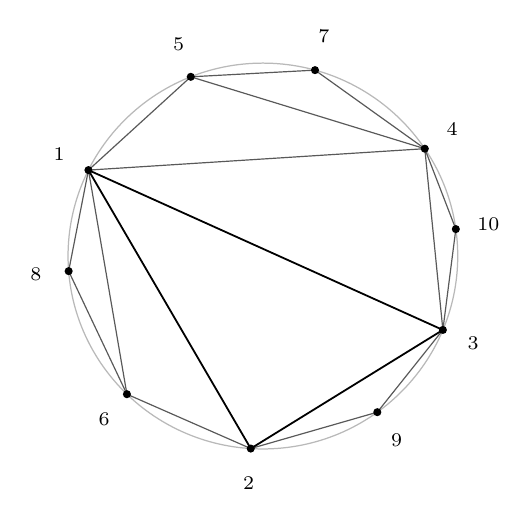
\begin{tikzpicture}[scale=2.45,line cap=round]
\draw[gray!55,line width=.45pt] (0,0) ellipse (1.01 and 1);
\draw[line width=.43pt,gray!70!black] (1.0001181561747635,0.13954311464423648) -- (0.83925008589116513,0.55636102291278378);
\draw[line width=.43pt,gray!70!black] (1.0001181561747635,0.13954311464423648) -- (0.93293028640184124,-0.38313260088125107);
\draw[line width=.43pt,gray!70!black] (0.83925008589116513,0.55636102291278378) -- (0.27017381691083328,0.96355818541719296);
\draw[line width=.43pt,gray!70!black] (0.83925008589116513,0.55636102291278378) -- (-0.3738826396647998,0.9289597150038693);
\draw[line width=.43pt,gray!70!black] (0.83925008589116513,0.55636102291278378) -- (-0.90429774889788693,0.44537464454187128);
\draw[line width=.43pt,gray!70!black] (0.83925008589116513,0.55636102291278378) -- (0.93293028640184124,-0.38313260088125107);
\draw[line width=.43pt,gray!70!black] (0.27017381691083328,0.96355818541719296) -- (-0.3738826396647998,0.9289597150038693);
\draw[line width=.43pt,gray!70!black] (-0.3738826396647998,0.9289597150038693) -- (-0.90429774889788693,0.44537464454187128);
\draw[line width=.43pt,gray!70!black] (-0.90429774889788693,0.44537464454187128) -- (-1.0068969956414558,-0.078327033470865103);
\draw[line width=.43pt,gray!70!black] (-0.90429774889788693,0.44537464454187128) -- (-0.70482680825359938,-0.71624556912397054);
\draw[line width=.65pt,black] (-0.90429774889788693,0.44537464454187128) -- (-0.062971999753061931,-0.99805443875887938);
\draw[line width=.65pt,black] (-0.90429774889788693,0.44537464454187128) -- (0.93293028640184124,-0.38313260088125107);
\draw[line width=.43pt,gray!70!black] (-1.0068969956414558,-0.078327033470865103) -- (-0.70482680825359938,-0.71624556912397054);
\draw[line width=.43pt,gray!70!black] (-0.70482680825359938,-0.71624556912397054) -- (-0.062971999753061931,-0.99805443875887938);
\draw[line width=.43pt,gray!70!black] (-0.062971999753061931,-0.99805443875887938) -- (0.593084843887274,-0.8094326564466194);
\draw[line width=.65pt,black] (-0.062971999753061931,-0.99805443875887938) -- (0.93293028640184124,-0.38313260088125107);
\draw[line width=.43pt,gray!70!black] (0.593084843887274,-0.8094326564466194) -- (0.93293028640184124,-0.38313260088125107);
\fill (1.0001181561747635,0.13954311464423648) circle (0.021);\node[fill=white,inner sep=1pt,font=\scriptsize] at (1.1684548755309118,0.16466087528019904) {10};
\fill (0.83925008589116513,0.55636102291278378) circle (0.021);\node[fill=white,inner sep=1pt,font=\scriptsize] at (0.98051000133819287,0.65650600703708482) {4};
\fill (0.27017381691083328,0.96355818541719296) circle (0.021);\node[fill=white,inner sep=1pt,font=\scriptsize] at (0.31564861777701312,1.1369986587922876) {7};
\fill (-0.3738826396647998,0.9289597150038693) circle (0.021);\node[fill=white,inner sep=1pt,font=\scriptsize] at (-0.43681338099451855,1.0961724637045657) {5};
\fill (-0.90429774889788693,0.44537464454187128) circle (0.021);\node[fill=white,inner sep=1pt,font=\scriptsize] at (-1.0565062808906005,0.52554208055940808) {1};
\fill (-1.0068969956414558,-0.078327033470865103) circle (0.021);\node[fill=white,inner sep=1pt,font=\scriptsize] at (-1.1763747077791265,-0.092425899495620817) {8};
\fill (-0.70482680825359938,-0.71624556912397054) circle (0.021);\node[fill=white,inner sep=1pt,font=\scriptsize] at (-0.82346102350420518,-0.8451697715662852) {6};
\fill (-0.062971999753061931,-0.99805443875887938) circle (0.021);\node[fill=white,inner sep=1pt,font=\scriptsize] at (-0.073571247236250569,-1.1777042377354776) {2};
\fill (0.593084843887274,-0.8094326564466194) circle (0.021);\node[fill=white,inner sep=1pt,font=\scriptsize] at (0.69291100572968641,-0.95513053460701084) {9};
\fill (0.93293028640184124,-0.38313260088125107) circle (0.021);\node[fill=white,inner sep=1pt,font=\scriptsize] at (1.0899581563902699,-0.45209646903987624) {3};
\end{tikzpicture}

\caption{A \emph{validated} ten-site construction on the noncircular ellipse $a/b=101/100$. Labels $1$--$10$ give arrival order. The first triangle is drawn more boldly; all other segments are the two \emph{compulsory} nearest-predecessor edges at their respective arrivals, never chosen as optional noncrossing diagonals. All $2n-3=17$ edges have been retained. A deterministic 80-decimal-place checker confirms each nearest-two choice and checks every independent edge pair for proper crossing; see \texttt{scripts/figure-validation.json}.}\label{fig:headline}
\end{figure}

Three features merit emphasis: the nearest sites are selected among \emph{earlier}, not all, vertices; the conclusion applies to arbitrarily many arbitrarily close distinct sites; and the sufficient interval of allowed aspect ratios is closed. Moreover, the proof is algorithmic: the order can be recovered by recursive metric-ear deletion in $O(n\log n)$ time (Section~\ref{sec:algorithm}). The argument relies on choosing a minimum \emph{Euclidean skip chord} among certain short two-gap arcs, not on simply removing the smallest angular gap. The latter tempting selection rule is false even at ratio $101/100$ (Section~\ref{sec:heuristic}).

The construction builds a maximal outerplanar graph on the boundary sites. Standard convex-polygon triangulation and greedy edge selection are classical, but they do not impose this particular mandatory predecessor rule. Relevant, distinct models include ordered one-nearest-neighbour graphs \citep{agoston2026}, ordered $\Theta$-graphs \citep{bose2004}, and greedy polygon triangulations \citep{levcopoulos1987,finlayson1992}. We do not claim the classical polygon-ear or outerplanar facts as original. A comprehensive historical priority determination has not been completed.

\section{The insertion model and finite-set foundations}\label{sec:model}
\begin{definition}[Chronological nearest-two drawing]\label{def:grow}
For a finite set $S$ of distinct points of the plane, choose a listing $(p_1,\dots,p_n)$ without repetition, $n\ge3$. Begin with all three sides of the triangle $p_1p_2p_3$. For $k=4,\dots,n$ rank $p_1,\dots,p_{k-1}$ by the pair
\[
 \bigl(\dist{p_k}{p_j}^{\,2},\ (p_j)_x,\ (p_j)_y\bigr)
\]
in ascending lexicographic order and connect $p_k$ to precisely the first two. Keep all earlier edges. Call this a \emph{plane nearest-two order} if no two open segments belonging to independent edges meet (equivalently, no proper crossing when no three sites are collinear).
\end{definition}

Lexicographic comparison makes the operation deterministic even when predecessor distances tie. The use of squared Euclidean distances changes no ranking. Ellipse-boundary sites have no collinear triple, because a line meets a nondegenerate ellipse in at most two points.

\begin{proposition}[Every three- or four-site set]\label{prop:four}
Every set $S$ of three or four distinct planar points with no three collinear admits a plane nearest-two order.
\end{proposition}
\begin{proof}
The three-site case is the initial triangle. If $|S|=4$ and a point $D$ lies inside the triangle on the other three vertices $A,B,C$, insert $D$ last: the two prescribed spokes from $D$ lie inside that triangle and cannot cross a side or one another.

Otherwise $S$ is a strictly convex quadrilateral $A,B,C,D$, named in cyclic order. Its diagonals $AC$ and $BD$ meet at $O$. Let $X$ be a vertex maximizing $\dist{X}{O}$; relabel cyclically so that $X=A$ and $C$ is opposite $A$. Strict triangle inequalities give
\[
 \dist{C}{B}<\dist{C}{O}+\dist{O}{B}
 \le\dist{C}{O}+\dist{O}{A}=\dist{C}{A}
\]
and likewise $\dist{C}{D}<\dist{C}{A}$. Thus the two closest predecessors of $C$ in $(A,B,D)$ are exactly $B,D$, regardless of their mutual distance tie. Start from triangle $ABD$ and insert $C$. Its two new edges are hull sides, so no crossing occurs.
\end{proof}

\begin{figure}[ht]
\centering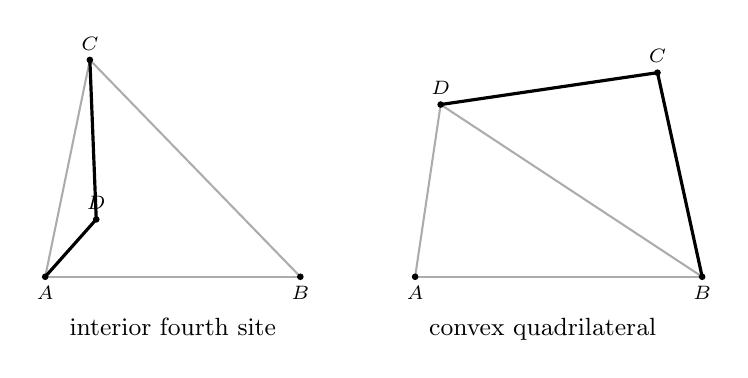
\begin{tikzpicture}[x=.81cm,y=.81cm,line cap=round]
\draw[gray!65,line width=.75pt] (0,0) -- (4,0);
\draw[gray!65,line width=.75pt] (4,0) -- (0.7,3.4);
\draw[gray!65,line width=.75pt] (0.7,3.4) -- (0,0);
\draw[black,line width=1.15pt] (0.8,0.9) -- (0,0);
\draw[black,line width=1.15pt] (0.8,0.9) -- (0.7,3.4);
\fill (0,0) circle (.052);\node[below,font=\scriptsize] at (0,0) {$A$};
\fill (4,0) circle (.052);\node[below,font=\scriptsize] at (4,0) {$B$};
\fill (0.7,3.4) circle (.052);\node[above,font=\scriptsize] at (0.7,3.4) {$C$};
\fill (0.8,0.9) circle (.052);\node[above,font=\scriptsize] at (0.8,0.9) {$D$};
\node[below,font=\small] at (2,-0.50) {interior fourth site};
\draw[gray!65,line width=.75pt] (5.8,0) -- (10.3,0);
\draw[gray!65,line width=.75pt] (10.3,0) -- (6.2,2.7);
\draw[gray!65,line width=.75pt] (6.2,2.7) -- (5.8,0);
\draw[black,line width=1.15pt] (9.6,3.2) -- (10.3,0);
\draw[black,line width=1.15pt] (9.6,3.2) -- (6.2,2.7);
\fill (5.8,0) circle (.052);\node[below,font=\scriptsize] at (5.8,0) {$A$};
\fill (10.3,0) circle (.052);\node[below,font=\scriptsize] at (10.3,0) {$B$};
\fill (9.6,3.2) circle (.052);\node[above,font=\scriptsize] at (9.6,3.2) {$C$};
\fill (6.2,2.7) circle (.052);\node[above,font=\scriptsize] at (6.2,2.7) {$D$};
\node[below,font=\small] at (7.8,-0.50) {convex quadrilateral};
\end{tikzpicture}

\caption{The general four-site base case, \emph{not} limited to ellipses. Left: an interior $D$ is inserted after triangle $ABC$; its forced neighbours are $A,C$. Right: a strictly convex quadrilateral permits triangle $ABD$ followed by $C$, whose forced neighbours are $B,D$. Black thick strokes show new edges and lighter strokes the seed triangle; the particular coordinates are validated in the figure script.}\label{fig:four}
\end{figure}

For strictly convex sets, every vertex is on the boundary of its convex hull, and its two \emph{cyclic neighbours} are the preceding and succeeding vertices around that hull.

\begin{definition}[Metric ear and full ear certificate]\label{def:ear}
Let $S$ be a finite set of at least four points in strictly convex position. A site $v\in S$ is a \emph{metric ear} if its two cyclic neighbours are exactly the first two sites in the lexicographically tie-broken distance ranking of $S\setminus\{v\}$ from $v$. A \emph{full metric-ear certificate} is a sequence of deletions, one such ear at each stage of size at least four, ending with three sites. A \emph{strict metric ear} has each adjacent site strictly closer to $v$ than every non-neighbour.
\end{definition}

\begin{theorem}[Recursive metric-ear characterisation]\label{thm:iff}
For every finite $S$ in strictly convex position with $|S|\ge3$, a plane nearest-two order exists if and only if a full metric-ear certificate exists.
\end{theorem}
\begin{proof}
For an order of $m$ sites, the seed contributes three edges and every subsequent insertion adds two distinct fresh edges, yielding exactly $2m-3$ edges. On $m$ strictly convex vertices a noncrossing graph has at most $2m-3$ edges: the polygon boundary plus at most $m-3$ interior diagonals in a triangulation. Moreover, if a boundary side were missing, it could be added without any crossing, contradicting the $2m-3$ cap. Thus all polygon sides already occur.

For $m\ge4$, consider the last vertex $v$ of an existing order. It has exactly its two insertion edges, since earlier insertions cannot be incident to it and there are no later insertions. Both hull sides at $v$ occur, so those two edges must join its immediate cyclic neighbours. By the insertion rule, this is a metric ear. Deleting $v$ preserves the previous valid nearest-two chronological construction on the remaining vertices. Iterating proves the necessary full certificate.

Conversely, take the last deletion of a full certificate as the initial triangle, and reverse the deletions. At each reinsertion the designated ear $v$ has exactly its two cyclic neighbours as nearest earlier sites. Those two segments are boundary sides of the enlarged convex polygon; previously drawn edges lie inside the smaller polygon. Thus neither new side crosses an old edge. The complete reversed sequence is the required order.
\end{proof}

\begin{figure}[ht]
\centering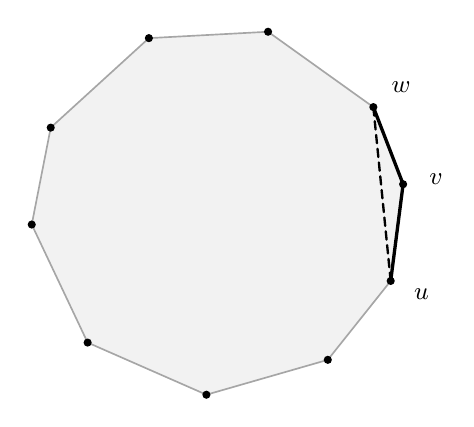
\begin{tikzpicture}[scale=2.35,line cap=round]
\fill[gray!10] (1.0001181561747635,0.13954311464423648) -- (0.83925008589116513,0.55636102291278378) -- (0.27017381691083328,0.96355818541719296) -- (-0.3738826396647998,0.9289597150038693) -- (-0.90429774889788693,0.44537464454187128) -- (-1.0068969956414558,-0.078327033470865103) -- (-0.70482680825359938,-0.71624556912397054) -- (-0.062971999753061931,-0.99805443875887938) -- (0.593084843887274,-0.8094326564466194) -- (0.93293028640184124,-0.38313260088125107) -- cycle;\draw[gray!70,line width=.6pt] (1.0001181561747635,0.13954311464423648) -- (0.83925008589116513,0.55636102291278378) -- (0.27017381691083328,0.96355818541719296) -- (-0.3738826396647998,0.9289597150038693) -- (-0.90429774889788693,0.44537464454187128) -- (-1.0068969956414558,-0.078327033470865103) -- (-0.70482680825359938,-0.71624556912397054) -- (-0.062971999753061931,-0.99805443875887938) -- (0.593084843887274,-0.8094326564466194) -- (0.93293028640184124,-0.38313260088125107) -- cycle;
\draw[very thick] (1.0001181561747635,0.13954311464423648) -- (0.93293028640184124,-0.38313260088125107);\draw[very thick] (1.0001181561747635,0.13954311464423648) -- (0.83925008589116513,0.55636102291278378);
\draw[densely dashed,line width=.85pt] (0.93293028640184124,-0.38313260088125107) -- (0.83925008589116513,0.55636102291278378);
\fill (1.0001181561747635,0.13954311464423648) circle (.022);\node[fill=white,inner sep=1.2pt,font=\small] at (1.1783570354930382,0.16605630642664141) {$v$};
\fill (0.83925008589116513,0.55636102291278378) circle (.022);\node[fill=white,inner sep=1.2pt,font=\small] at (0.98881940812919452,0.66206961726621266) {$w$};
\fill (0.27017381691083328,0.96355818541719296) circle (.022);
\fill (-0.3738826396647998,0.9289597150038693) circle (.022);
\fill (-0.90429774889788693,0.44537464454187128) circle (.022);
\fill (-1.0068969956414558,-0.078327033470865103) circle (.022);
\fill (-0.70482680825359938,-0.71624556912397054) circle (.022);
\fill (-0.062971999753061931,-0.99805443875887938) circle (.022);
\fill (0.593084843887274,-0.8094326564466194) circle (.022);
\fill (0.93293028640184124,-0.38313260088125107) circle (.022);\node[fill=white,inner sep=1.2pt,font=\small] at (1.099195089919001,-0.45592779504868875) {$u$};
\end{tikzpicture}

\caption{A strict metric ear $v$ (thick incident sides) in a seven-or-more-site cyclic subset of the validated ten-site example. Its cyclic neighbours are $u,w$; the dashed skip chord $uw$ becomes a hull side when $v$ is removed. The strict nearest-two condition means $\dist{v}{u},\dist{v}{w}<\dist{v}{z}$ for every other remaining site $z$. Reversing removal adds exactly $vu,vw$ without disturbing old edges.}\label{fig:ear}
\end{figure}

\section{Ellipse chords and the short-arc cutoff}\label{sec:derivative}
Set $P(t)=(a\cos t,b\sin t)$, $a\ge b>0$, and define
\begin{equation}\label{eq:lambda}
 M=\frac{a^2+b^2}{2},\quad D=\frac{a^2-b^2}{2},\qquad
 \Lambda=4\arctan\frac ba=2\arccos\frac DM\in(0,\pi].
\end{equation}
Let $\theta<\phi$ be a real, \emph{unwrapped} parameter pair and put $\Delta=\phi-\theta$. The squared chord has the exact expression
\begin{equation}\label{eq:chord}
 F(\theta,\phi)=\dist{P(\theta)}{P(\phi)}^2
 =4\sin^2(\Delta/2)\,[M-D\cos(\theta+\phi)].
\end{equation}

\begin{lemma}[Both signed derivatives and strict short-arc extension]\label{lem:short}
Whenever $0<\Delta<\Lambda$,
\begin{align}
 \partial_\phi F(\theta,\phi)
 &=4\sin(\Delta/2)\left[M\cos(\Delta/2)-D\cos\frac{\theta+3\phi}{2}\right]>0,\label{eq:right}\\[1mm]
 -\partial_\theta F(\theta,\phi)
 &=4\sin(\Delta/2)\left[M\cos(\Delta/2)-D\cos\frac{3\theta+\phi}{2}\right]>0.\label{eq:left}
\end{align}
In particular, if $\theta_0\le\theta_1<\phi_0\le\phi_1$, at least one outer extension is nontrivial, and $\phi_1-\theta_0<\Lambda$, then
\[
 \dist{P(\theta_1)}{P(\phi_0)}
 <\dist{P(\theta_0)}{P(\phi_1)}.
\]
The same strict inequality holds for squared chord lengths.
\end{lemma}
\begin{proof}
Differentiate \eqref{eq:chord} in each endpoint, noting the negative sign when the left endpoint moves outward (left). Since $\Delta<\Lambda=2\arccos(D/M)$, we have $\cos(\Delta/2)>D/M$, whereas either phase cosine is at most one. Both displayed brackets are therefore strictly positive. Integrating one or both signed derivatives along the relevant real-lift endpoint extension proves strict growth. This argument does not require that the lifted interval lie inside $[0,2\pi)$.
\end{proof}

At $\Delta=\Lambda$ the derivative can cease to be \emph{strictly} positive; we shall put both angular boundary cases into a separate closed central range, rather than using an unjustified endpoint extension.

\section{A strict metric ear at every cardinality}\label{sec:earproof}
The essential geometric statement is the following.
\begin{lemma}[Uniform ellipse metric ear]\label{lem:uniform}
Suppose $m\ge5$, $0<b\le a$, $a/b\le\Rbound$, and $S\subset\Ell$ consists of $m$ distinct points. Then $S$ has a strict metric ear, without a minimum-spacing assumption.
\end{lemma}
\begin{proof}
List the sites cyclically $v_i=P(\theta_i)$, with indices taken modulo $m$. Work on a cyclic real lift, so the positive consecutive gaps $g_i$ sum to $2\pi$. For each $i$ define the adjacent two-gap span and Euclidean skip chord
\[
 s_i=g_{i-1}+g_i,\qquad L_i=\dist{v_{i-1}}{v_{i+1}}.
\]
Every $g_i$ enters two of the $s_j$, so
\begin{equation}\label{eq:average}
 \sum_{i=1}^{m}s_i=4\pi,
 \qquad\min_i s_i\le\frac{4\pi}{m}\le\frac{4\pi}{5}.
\end{equation}
The cutoff is strictly above this benchmark \emph{even at the claimed endpoint}. Indeed,
\[
 \Rbound<\cot(\pi/5),\qquad
 \frac ab\le\Rbound\quad\Longrightarrow\quad
 \Lambda=4\arctan(b/a)>\frac{4\pi}{5}.
\]
The first inequality follows from $\sin(\pi/5)<\cos(\pi/5)$ after squaring the positive terms. Hence the finite eligible index set $I=\{i:s_i<\Lambda\}$ is nonempty. Choose $i\in I$ to minimise \emph{$L_i$ among eligible indices}. This is a metric minimisation, not selection of the smallest $s_i$.

Both adjacent chords $v_iv_{i-1}$ and $v_iv_{i+1}$ are strictly shorter than $L_i$ by Lemma~\ref{lem:short}: their arcs are proper subarcs of the eligible span $s_i<\Lambda$. We claim
\begin{equation}\label{eq:ear}
 \dist{v_i}{v_{i-1}},\ \dist{v_i}{v_{i+1}}<L_i
 \le\dist{v_i}{v_j}\qquad (j\notin\{i-1,i,i+1\}).
\end{equation}

Fix any non-neighbour $v_j$ and let $\delta\in(0,2\pi)$ be its forward parameter separation from $v_i$. We divide competitors into three disjoint ranges, assigning equality endpoints to the central range (Figure~\ref{fig:bands}).

\begin{figure}[ht]
\centering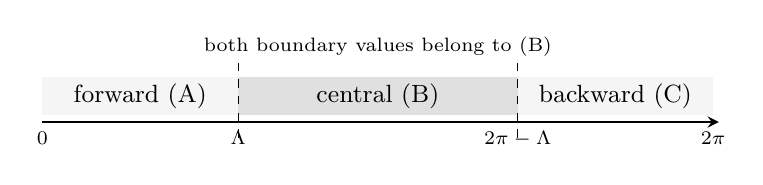
\begin{tikzpicture}[x=0.71cm,y=0.71cm,>=stealth]
\draw[thick,->] (0,0) -- (12.1,0);
\fill[gray!8] (0,0.12) rectangle (3.5,.8);
\fill[gray!24] (3.5,.12) rectangle (8.5,.8);
\fill[gray!8] (8.5,.12) rectangle (12,.8);
\draw[dashed] (3.5,-.28) -- (3.5,1.1);
\draw[dashed] (8.5,-.28) -- (8.5,1.1);
\node[font=\small] at (1.75,.46) {forward (A)};
\node[font=\small] at (6,.46) {central (B)};
\node[font=\small] at (10.25,.46) {backward (C)};
\node[below,font=\scriptsize] at (0,0) {$0$};
\node[below,font=\scriptsize] at (3.5,0) {$\Lambda$};
\node[below,font=\scriptsize] at (8.5,0) {$2\pi-\Lambda$};
\node[below,font=\scriptsize] at (12,0) {$2\pi$};
\node[above,font=\scriptsize] at (6,1.0) {both boundary values belong to (B)};
\end{tikzpicture}

\caption{The three competitor regimes measured \emph{forward} from $v_i$. Range (A) is $0<\delta<\Lambda$, range (B) is the \emph{closed} interval $\Lambda\le\delta\le2\pi-\Lambda$, and range (C) is $2\pi-\Lambda<\delta<2\pi$. The diagram is an affine schematic of angular intervals, not a drawing to true angular scale. At the circle $\Lambda=\pi$, (B) consists of the single antipodal parameter difference.}\label{fig:bands}
\end{figure}

\emph{Forward short range} $0<\delta<\Lambda$. As $j$ is not the next cyclic site, the arc from $i$ to $j$ includes $v_{i+2}$, and $s_{i+1}\le\delta<\Lambda$. Thus $i+1\in I$, and extension with $v_i$ fixed gives
\begin{equation}\label{eq:fwd}
 \dist{v_i}{v_j}\ge\dist{v_i}{v_{i+2}}
 =L_{i+1}\ge L_i.
\end{equation}
Equality in the first comparison is allowed when $j=i+2$. The last inequality is by our eligible minimum.

\emph{Backward short range} $2\pi-\Lambda<\delta<2\pi$. The backward arc has width $2\pi-\delta<\Lambda$. As $j$ is not the previous cyclic site, this arc passes $v_{i-2}$; $s_{i-1}<\Lambda$ and the independent \emph{left-endpoint} extension yields
\begin{equation}\label{eq:back}
 \dist{v_i}{v_j}\ge\dist{v_i}{v_{i-2}}
 =L_{i-1}\ge L_i.
\end{equation}
These comparisons stay in their own short directions; no false comparison of chords spanning opposite arcs is used.

\emph{Central closed range} $\Lambda\le\delta\le2\pi-\Lambda$. Ellipse scaling from the unit circle yields the lower bound
\begin{equation}\label{eq:central}
 \dist{v_i}{v_j}\ge2b\sin(\delta/2)
 \ge2b\sin(\Lambda/2)=\frac{4ab^2}{a^2+b^2}.
\end{equation}
(The sine minimum over the symmetric closed central interval occurs at an endpoint.) Let $j_0$ realise the averaging bound \eqref{eq:average}. Since $s_{j_0}\le4\pi/5<\Lambda$, it is eligible. Ellipse scaling also bounds its Euclidean skip chord by a major-axis-scaled circle chord:
\begin{equation}\label{eq:skip}
 L_i\le L_{j_0}\le2a\sin(s_{j_0}/2)
 \le2a\sin(2\pi/5).
\end{equation}
Finally, the hypothesis $r=a/b\le\Rbound$ gives
\begin{equation}\label{eq:keyineq}
 r^2+1\le\Rbound^2+1=\frac{2}{\sin(2\pi/5)}
 \quad\Longleftrightarrow\quad
 2a\sin(2\pi/5)\le\frac{4ab^2}{a^2+b^2}.
\end{equation}
Combining \eqref{eq:central}--\eqref{eq:keyineq} proves $\dist{v_i}{v_j}\ge L_i$ in the whole central interval, \emph{including} $\delta=\Lambda,2\pi-\Lambda$ and $a/b=\Rbound$.

All non-neighbours therefore satisfy \eqref{eq:ear}, while both neighbours lie \emph{strictly} below $L_i$. They are the compulsory two nearest predecessors (whatever ties occur among the other sites). Thus $v_i$ is a strict metric ear.
\end{proof}

\begin{proof}[Proof of Theorem~\ref{thm:ellipse}]
Every finite distinct boundary subset is strictly convex. At each stage with at least five surviving sites, Lemma~\ref{lem:uniform} produces a strict metric ear on the \emph{same} ellipse, independent of the number or spacing of the survivors. Delete and repeat to four points, use Proposition~\ref{prop:four} for the final four-site order, and reverse the metric-ear deletions. Each reverse insertion uses precisely its two nearest earlier neighbours and adds only boundary sides; no old edges are removed and no proper crossing occurs. The full recursive certificate criterion in Theorem~\ref{thm:iff} gives the equivalent formulation. The closed ratio endpoint has already been used in \eqref{eq:keyineq}.
\end{proof}


\section{Constructing the order efficiently}\label{sec:algorithm}
The metric-ear proof is constructive, not merely existential. In the notation of Lemma~\ref{lem:uniform}, an eligible site is one whose current cyclic-neighbour span satisfies $s_i<\Lambda$, and its priority is the squared Euclidean skip-chord length $L_i^2=\dist{v_{i-1}}{v_{i+1}}^2$. The squared length gives the same minimisers as $L_i$ and avoids square roots.

\begin{proposition}[Algorithmic corollary]\label{prop:algorithm}
Given $a\ge b>0$ with $a/b\le\Rbound$ and $n\ge3$ distinct Cartesian-coordinate sites on $\Ell$, a plane nearest-two order can be constructed in $O(n\log n)$ time and $O(n)$ auxiliary space in the exact real-arithmetic comparison model.
\end{proposition}

\noindent\textbf{Algorithm (cyclic ear deletion and reversal).}
\begin{enumerate}[leftmargin=*,itemsep=1pt,topsep=3pt]
\item Sort the sites cyclically about the ellipse centre and put them into a circular doubly linked list.
\item For each site in the current list, test eligibility $s_i<\Lambda$. Insert each eligible site into a min-priority queue keyed by $L_i^2$, breaking equal keys by Cartesian-lexicographic site coordinates.
\item While more than four sites survive, extract a minimum-key eligible site $v_i$, record it, and delete it from the circular list. Recompute eligibility and priority for its two surviving cyclic neighbours, updating their queue entries. Invalidated entries may instead be discarded lazily using version counters.
\item Order the final three or four sites by Proposition~\ref{prop:four}, then append the recorded deleted sites in reverse deletion order.
\end{enumerate}

\begin{proof}
For every stage with at least five sites, equation~\eqref{eq:average} guarantees an eligible index. Lemma~\ref{lem:uniform} proves that a minimum Euclidean skip-chord candidate \emph{among eligible sites} is a strict metric ear. Thus step~3 always finds a valid deletion. The remaining set lies on the same ellipse and satisfies the same aspect-ratio bound. Proposition~\ref{prop:four} constructs the base order, and reversing the deletions inserts only the compulsory nearest-two hull sides, without crossing an old edge. Heap tie-breaking affects only which valid ear is removed; strictness relative to non-neighbours makes distance ties harmless.

It remains to justify the running time without assuming an angular oracle. Write $q_i=((v_i)_x/a,(v_i)_y/b)$, so $q_i$ lies on the unit circle, and put
\[
 c_\Lambda=\cos\Lambda
 =2\left(\frac{a^2-b^2}{a^2+b^2}\right)^2-1.
\]
Because $0<\Lambda\le\pi$ and $0<s_i<2\pi$, the eligibility test is exactly
\begin{equation}\label{eq:algebraic-eligibility}
 s_i<\Lambda
 \quad\Longleftrightarrow\quad
 \det(q_{i-1},q_{i+1})>0
 \ \text{and}\ 
 q_{i-1}\mathbin{\cdot}q_{i+1}>c_\Lambda.
\end{equation}
The determinant specifies the positively oriented arc of length less than $\pi$, and the dot product gives the remaining strict cutoff. In particular, equality at $s_i=\Lambda$ is \emph{ineligible}, as in the proof above. The initial cyclic sort can likewise be carried out with half-plane and determinant comparisons, without evaluating inverse trigonometric functions. All these tests, and the squared-distance priorities, use a constant number of exact real-arithmetic operations and comparisons.

Deleting $v_i$ changes the cyclic neighbours, hence the eligibility and priority, of only its immediate surviving predecessor and successor. Each of the at most $n-4$ deletions therefore causes $O(1)$ queue updates. There are $O(n)$ total queue insertions and removals, each costing $O(\log n)$, and the initial cyclic sort costs $O(n\log n)$. The final three- or four-site construction and the reversal cost $O(n)$ overall. The linked list, queue, deletion stack and output order each use $O(n)$ space. This is an exact real-arithmetic bound; no bit-complexity claim is made for arbitrary real input coordinates.
\end{proof}

\section{A noncircular universal corollary}\label{sec:corollary}
\begin{corollary}\label{cor:nonround}
On the noncircular ellipse $E(101/100,1)$, \emph{every} finite set of at least three distinct boundary sites admits a plane nearest-two order.
\end{corollary}
\begin{proof}
The identity $\sin^2(2\pi/5)=(5+\sqrt5)/8$ gives
$\sin(2\pi/5)<39/40<20000/20201=2/(1+(101/100)^2)$.
Hence $1<101/100<\Rbound$, and Theorem~\ref{thm:ellipse} applies.
\end{proof}

\section{Why minimising angular span is not enough}\label{sec:heuristic}
The proof requires \emph{metric} skip-chord minimisation over the eligible indices. Here is a concrete obstruction to the rule ``always delete the site with least adjacent angular two-gap''; it is \emph{not} a counterexample to Theorem~\ref{thm:ellipse}.

On the ellipse $E(101/100,1)$, use rational half-angle coordinates
\[
 Q(t)=\left(\frac{101}{100}\frac{1-t^2}{1+t^2},\frac{2t}{1+t^2}\right)
\]
and cyclic sites $P_0=Q(0)$, $P_1=Q(1/3)$, $P_2=Q(9/4)$, $P_3=Q(113/50)$, $P_4=Q(-9/4)$. Their increasing unwrapped angles are
\[
 0,\quad 2\arctan(1/3),\quad2\arctan(9/4),\quad
 2\arctan(113/50),\quad2\pi-2\arctan(9/4).
\]
The adjacent two-gap sums $s_i$ have the \emph{unique} minimum at $i=2$: comparing the relevant positive half-angle arctangents reduces the close case $s_2<s_3$ to $289\cdot65=18785<18936=72\cdot263$; the other three comparisons are immediate from their displayed angular positions and $s_4>\pi$. Yet $P_2$ is not a metric ear, since the non-neighbour $P_4$ is closer than cyclic neighbour $P_1$:
\begin{equation}\label{eq:obstruction}
 \dist{P_2}{P_1}^2-\dist{P_2}{P_4}^2
 =\frac{49482169}{2352250000}>0.
\end{equation}

\begin{figure}[ht]
\centering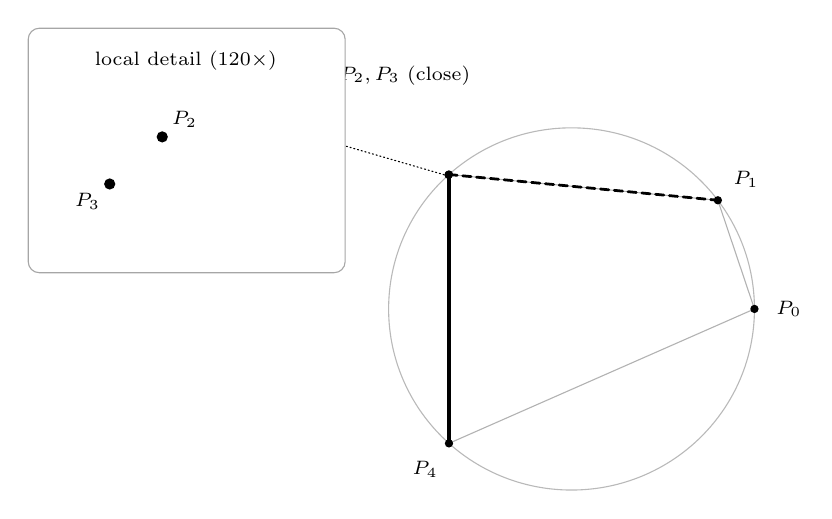
\begin{tikzpicture}[scale=2.30,line cap=round]
\draw[gray!55] (0,0) ellipse (1.01 and 1);
\draw[gray!60] (1.01,0.0) -- (0.808,0.6) -- (-0.67680412371134021,0.7422680412371134) -- (-0.6792645228895147,0.74006156264326413) -- (-0.67680412371134021,-0.7422680412371134) -- cycle;
\draw[very thick] (-0.67680412371134021,0.7422680412371134) -- (-0.67680412371134021,-0.7422680412371134);
\draw[densely dashed,line width=1.0pt] (-0.67680412371134021,0.7422680412371134) -- (0.808,0.6);
\fill (1.01,0.0) circle (.023);
\node[font=\scriptsize,fill=white,inner sep=1pt] at (1.2,0.0) {$P_0$};
\fill (0.808,0.6) circle (.023);
\node[font=\scriptsize,fill=white,inner sep=1pt] at (0.96342306439642318,0.71541316663100731) {$P_1$};
\fill (-0.67680412371134021,0.7422680412371134) circle (.023);
\fill (-0.6792645228895147,0.74006156264326413) circle (.023);
\fill (-0.67680412371134021,-0.7422680412371134) circle (.023);
\node[font=\scriptsize,fill=white,inner sep=1pt] at (-0.80852440857428697,-0.88672897817743583) {$P_4$};
\node[font=\scriptsize,fill=white,inner sep=1pt] at (-.92,1.29) {$P_2,P_3$ (close)};
\draw[densely dotted] (-.683,.735) -- (-1.25,.9);
\draw[gray!70,rounded corners,fill=white] (-3.0,.20) rectangle (-1.25,1.55);
\node[font=\scriptsize] at (-2.13,1.37) {local detail ($120\times$)};
\fill (-2.26,.95) circle (.031);
\fill (-2.55,.69) circle (.031);
\node[font=\scriptsize,above right] at (-2.26,.95) {$P_2$};
\node[font=\scriptsize,below left] at (-2.55,.69) {$P_3$};
\end{tikzpicture}

\caption{Five-site counterexample to the \emph{minimum-angular-two-gap ear-selection heuristic}, not to the paper's existence theorem. The unique two-gap minimiser $P_2$ has a closer \emph{non-neighbour} $P_4$ (solid chord) than its neighbour $P_1$ (dashed chord). All sites use exact rational coordinates; the strict squared-distance difference is given in \eqref{eq:obstruction}. Other vertices in this set are valid metric ears.}\label{fig:obstruction}
\end{figure}

This example explains why averaging angular gaps alone does not identify an ear. Averaging is used to guarantee an eligible set and to bound a particular witness skip chord, after which the minimum is taken in \emph{Euclidean length}.

\section{Verification, context and limitations}\label{sec:verify}
The five precise mathematical statements have direct proofs in the public Lean namespace \texttt{ETSHTS}. The original direct declaration names and proof modules are
\begin{center}\small
\begin{tabular}{@{}ll@{}}\toprule
\textbf{Exact theorem} & \textbf{Proof module} \\\midrule
\texttt{clm0096\_exact} & \texttt{ConvexFourClassification.lean}\\
\texttt{clm0099\_exact} & \texttt{GenuineOuterplanarCap.lean}\\
\texttt{clm0102\_exact} & \texttt{Cutoff.lean}\\
\texttt{clm0107\_exact} & \texttt{CyclicCompetitorExact.lean}\\
\texttt{clm0108\_exact} & \texttt{ExactNonround.lean}\\\bottomrule
\end{tabular}
\end{center}
They formalise, respectively, Proposition~\ref{prop:four}, Theorem~\ref{thm:iff}, Lemma~\ref{lem:short}, Theorem~\ref{thm:ellipse}, and Corollary~\ref{cor:nonround}. The Lean semantics use real Cartesian points, squared Euclidean predecessor ranking with lexicographic ties, retained two-edge insertions, and open-segment planarity; see the machine-readable target definitions \citep{etshtsrepo}. The algorithmic running-time analysis in Proposition~\ref{prop:algorithm} is a paper-level corollary of the constructive metric-ear proof, not a separately certified Lean complexity theorem. These machine-checked proofs are distinct from historical originality, external mathematical peer review, or a Palomar-issued registration. \textbf{\PalomarRecordStatus.} A future verified versioned record will be linked at the single macro \verb|\PalomarRecordURL| once actually issued.

The bound $\Rbound$ is only a \emph{sufficient} closed range; the set of all successful aspect ratios, and sharpness of the displayed constant, are not settled here. Our recursion also does not assert a suitable order on arbitrary large convex site sets: the exact if-and-only-if ear certificate specifies when one exists. A previous internal literature review recorded an unresolved access gap concerning a 1992 convex greedy-triangulation paper and broader historical priority searches \citep{finlayson1992}. Citation overlap and proof priority require independent investigation; neither formalisation nor a successful local proof implies publication or external review.

\paragraph{Acknowledgements.} The author acknowledges the Lean and Mathlib communities and AI-assisted formalisation and drafting under the author's direction. No external referee review is claimed.

\begin{thebibliography}{9}
\bibitem[\'{A}goston et~al.(2026)]{agoston2026}
P.~\'{A}goston, A.~Dumitrescu, A.~Sagdeev, K.~Singh, and J.~Zeng.
\newblock Maximizing the maximum degree in ordered nearest neighbor graphs.
\newblock \emph{Computational Geometry}, 132:102229, 2026.
\newblock \href{https://doi.org/10.1016/j.comgeo.2025.102229}{doi:10.1016/j.comgeo.2025.102229}.
\bibitem[Bose et~al.(2004)]{bose2004}
P.~Bose, J.~Gudmundsson, and P.~Morin.
\newblock Ordered theta graphs.
\newblock \emph{Computational Geometry}, 28(1):11--18, 2004.
\newblock \href{https://doi.org/10.1016/j.comgeo.2004.01.003}{doi:10.1016/j.comgeo.2004.01.003}.
\bibitem[Levcopoulos and Lingas(1987)]{levcopoulos1987}
C.~Levcopoulos and A.~Lingas.
\newblock On approximation behavior of the greedy triangulation for convex polygons.
\newblock \emph{Algorithmica}, 2:175--193, 1987.
\newblock \href{https://doi.org/10.1007/BF01840358}{doi:10.1007/BF01840358}.
\bibitem[Finlayson and Bhattacharya(1992)]{finlayson1992}
G.~D.~Finlayson and B.~K.~Bhattacharya.
\newblock A practical algorithm for the greedy triangulation of a convex polygon.
\newblock In \emph{4th Canadian Conference on Computational Geometry}, pages 347--352, 1992.
\bibitem[Fairfax-Ball(2026)]{etshtsrepo}
J.~Fairfax-Ball.
\newblock \emph{Noncrossing Two-Nearest-Predecessor Orders on Nearly Circular Ellipses:
Lean 4 Sources and Proof Archive}.
\newblock \url{https://github.com/jfairfaxball-348/ellipse-theorem}, 2026.
\end{thebibliography}
\end{document}
